\documentclass{InsightArticle}

\usepackage[dvips]{graphicx}
\usepackage{color}
\usepackage{listings}

\definecolor{listcomment}{rgb}{0.0,0.5,0.0}
\definecolor{listkeyword}{rgb}{0.0,0.0,0.5}
\definecolor{listnumbers}{gray}{0.65}
\definecolor{listlightgray}{gray}{0.955}
\definecolor{listwhite}{gray}{1.0}

\lstset{frame = tb,
       framerule = 0.25pt,
       float,
       fontadjust,
       backgroundcolor={\color{listlightgray}},
       basicstyle = {\ttfamily\footnotesize},
       keywordstyle = {\ttfamily\color{listkeyword}\textbf},
       identifierstyle = {\ttfamily},
       commentstyle = {\ttfamily\color{listcomment}\textit},
       stringstyle = {\ttfamily},
       showstringspaces = false,
       showtabs = false,
       numbers = left,
       numbersep = 6pt,
       numberstyle={\ttfamily\color{listnumbers}},
       tabsize = 2,
       language=[ANSI]C++,
       floatplacement=!h
       }

%%%%%%%%%%%%%%%%%%%%%%%%%%%%%%%%%%%%%%%%%%%%%%%%%%%%%%%%%%%%%%%%%%
%
%  hyperref should be the last package to be loaded.
%
%%%%%%%%%%%%%%%%%%%%%%%%%%%%%%%%%%%%%%%%%%%%%%%%%%%%%%%%%%%%%%%%%%
\usepackage[dvips,
bookmarks,
bookmarksopen,
backref,
colorlinks,linkcolor={blue},citecolor={blue},urlcolor={blue},
]{hyperref}


\title{Introduction to ITK Resample In-Place Image Filter}

%
% NOTE: This is the last number of the "handle" URL that
% The Insight Journal assigns to your paper as part of the
% submission process. Please replace the number "1338" with
% the actual handle number that you get assigned.
%
\newcommand{\IJhandlerIDnumber}{3224}

% Increment the release number whenever significant changes are made.
% The author and/or editor can define 'significant' however they like.
\release{0.00}

% At minimum, give your name and an email address.  You can include a
% snail-mail address if you like.
\author{Wei Lu$^{1}$, Hans Johnson$^{2}$$^{3}$}
\authoraddress{$^{1}$Department of Electrical and Computer Engineering, The University of Iowa\\
               $^{2}$Department of Psychiatry, The University of Iowa\\
               $^{3}$Department of Biomedical Engineering, The University of Iowa}

\begin{document}

%
% Add hyperlink to the web location and license of the paper.
% The argument of this command is the handler identifier given
% by the Insight Journal to this paper.
%
\IJhandlefooter{\IJhandlerIDnumber}


\ifpdf
\else
   %
   % Commands for including Graphics when using latex
   %
   \DeclareGraphicsExtensions{.eps,.jpg,.gif,.tiff,.bmp,.png}
   \DeclareGraphicsRule{.jpg}{eps}{.jpg.bb}{`convert #1 eps:-}
   \DeclareGraphicsRule{.gif}{eps}{.gif.bb}{`convert #1 eps:-}
   \DeclareGraphicsRule{.tiff}{eps}{.tiff.bb}{`convert #1 eps:-}
   \DeclareGraphicsRule{.bmp}{eps}{.bmp.bb}{`convert #1 eps:-}
   \DeclareGraphicsRule{.png}{eps}{.png.bb}{`convert #1 eps:-}
\fi


\maketitle


\ifhtml
\chapter*{Front Matter\label{front}}
\fi


% The abstract should be a paragraph or two long, and describe the
% scope of the document.
\begin{abstract}
\noindent
In this document we present an ITK
\cite{ITKSoftwareGuideSecondEdition} image filter that outputs a new
image with identical voxel contents but with modified physical space
representation. The physical space representation of an image is
modified to reflect the physical space transform on the input
image. The advantage of this filter is that it is free from
interpolation error.

This paper is accompanied with the source code, input data, parameters
and output data that the authors used for validating the algorithm
described in this paper. This adheres to the fundamental principle
that scientific publications must facilitate reproducibility of the
reported results.

\end{abstract}

\IJhandlenote{\IJhandlerIDnumber}

\tableofcontents

% Motivation
The current ITK resample image filter transforms, interpolates, and resamples an input image $I$ into a new voxel lattice and physical space specified by the programmer.   The newly created output image updates the voxel contents with interpolated values from the input image $I$.

A side effect of this process is that it introduces interpolation error, i.e., even given the inverse of the nontrivial input transform and the resampled image, it is generally impossible to obtain the original image. The problem can be even worse if several of resample filters are being used to generating intermediate output images in the entire process.

This filter takes advantage of the fact that the voxel lattice to physical space transform is represented as a rigid transform in ITK.  If all the transforms to be applied are rigid, then by composing the transforms before hand, we can achieve the desired physical space representation without accumulating interpolation errors.

\section{Principle}

An ITK image class has a rigid transform representation that maps a physical space coordinate system onto the discrete voxel lattice. The physical space representation includes the orientation matrix of the image $\mathbf{R_0}$, the origin vector of the image $\mathbf{T_0}$, and the spacing vector of the image $\mathbf{S_0}$. Thus each ITK image $\mathbf{I}$ can be represented as a composition of an image $\mathbf{I_0}$ with isotropic spacing, zero origin, and identity orientation, and an affine transform $\mathbf{A}$ by
\begin{equation}
\mathbf{I} = \mathbf{A}\mathbf{I_0}
\end{equation}
Where
\begin{eqnarray}
\label{equ-A}
\mathbf{A} & = & \mathbf{T_0}\mathbf{R_0}\mathbf{S_0} \nonumber \\
& = &
\left[ {\begin{array}{cc}
\mathbf{R_0}\mathbf{S_0} & \mathbf{T_0} \\
 & 1
\end{array} } \right]
\end{eqnarray}

Recall that a rigid transform matrix $\mathbf{M}$ is composed of a translation matrix $\mathbf{T}$ and a rotation matrix $\mathbf{R}$, \textit{i.e.},
\begin{eqnarray}
\mathbf{M} & = & \mathbf{T}\mathbf{R} \nonumber \\
& = &
\left[ {\begin{array}{cc}
\mathbf{R} & \mathbf{T} \\
 & 1
\end{array} } \right]
\end{eqnarray}

The output image $\mathbf{I_1}$ can be obtained by
\begin{equation}
\mathbf{I_1} = \mathbf{M}\mathbf{I} = (\mathbf{M}\mathbf{A})\mathbf{I_0}
\end{equation}

Therefore, we have the composed image info matrix
\begin{eqnarray}
\label{equ-M}
\mathbf{M}\mathbf{A} & = & \mathbf{T}\mathbf{R}\mathbf{T_0}\mathbf{R_0}\mathbf{S_0} \nonumber \\
& = &
\left[ {\begin{array}{cc}
(\mathbf{R}\mathbf{R_0})\mathbf{S_0} & \mathbf{R}\mathbf{T_0} + \mathbf{T} \\
 & 1
\end{array} } \right]
\end{eqnarray}

By contrasting \textbf{Equations} \ref{equ-A} and \ref{equ-M} we have
\begin{eqnarray}
\mathbf{T_1} & = & \mathbf{R}\mathbf{T_0} + \mathbf{T} \nonumber \\
\mathbf{R_1} & = & \mathbf{R}\mathbf{R_0} \nonumber \\
\mathbf{S_1} & = & \mathbf{S_0}
\end{eqnarray}

Where $\mathbf{T_1}$, $\mathbf{R_1}$, and $\mathbf{S_1}$ are the output image origin vector, orientation matrix, and spacing vector, respectively.

\section{Validation}

Assume we have an image $I_1$, which is centered at the origin of an LPS coordinate system, and a rigid transform $\mathbf{T}$ that will first translate the image $300$ mm along $-P$-axis, and then a $0.5$ rad rotation along $-L$-axis about the origin. The mid-sagittal plane of both the input image and the output image $I_2$ from the \textit{itkResampleInPlaceImageFilter} are shown in the same physical space but lie in their own index space in \textbf{Figure 2}. Also, we have labeled a distinctive landmark (\textit{ac}) for each image (\textit{i.e.}, the point $A$ in $I_1$ and the point $B$ in $I_2$). Their locations in index space and physical space are listed in \textbf{Table 1}.
\begin{figure}[htp]
	\begin{center}
		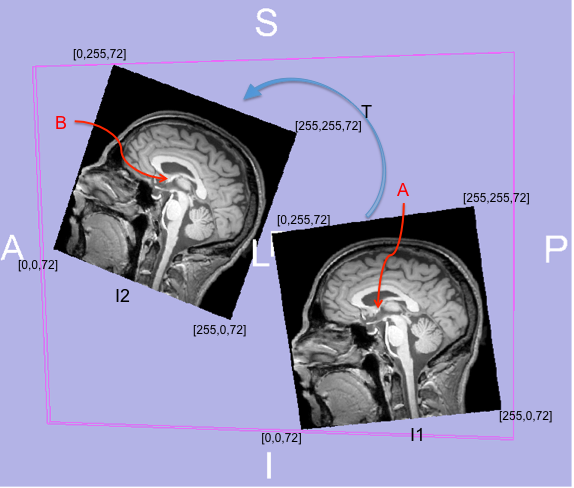
\includegraphics[width=0.7\textwidth]{itkResampleInPlaceImageFilter-Demo}
		\caption{Input image $I_1$ and the transformed output image $I_2$ are shown in the same physical space but lie in their own index space. The index extent are labeled in black for each image.}
	\end{center}
\end{figure}
\begin{table}[htbp]
\begin{center}
\begin{tabular}{ | p{3cm} | p{3cm} | p{3cm} | }
\hline
 & \textbf{Index space} & \textbf{Physical space} \\ \hline
\textbf{Input} ($A$) & [$119$, $141$, $72$] & ($0$, $29.0$, $19.4$) \\ \hline
\textbf{output} ($B$) & [$119$, $141$, $72$] & ($0$, $280.3$, $174.8$) \\ \hline
\end{tabular}
\end{center}
\caption{This table shows the ac locations in input/output and index/physical space. The output image has the same voxel contents as that of the input image but with different physical representation due to the impact of an input rigid transform.}
\end{table}

\section{Usage}

First include the header file by
\begin{center}
\lstinputlisting[linerange={23-23}]{../../Testing/Code/itkResampleInPlaceImageFilterTest.cxx}
\end{center}

Define the resample in-place image filter by
\begin{center}
\lstinputlisting[linerange={66-66}]{../../Testing/Code/itkResampleInPlaceImageFilterTest.cxx}
\end{center}

Set up the filter and process the input volume
\begin{center}
\lstinputlisting[linerange={99-103}]{../../Testing/Code/itkResampleInPlaceImageFilterTest.cxx}
\end{center}

%Acknowledgement
\section{Acknowledgement}

This research was supported by funding from grants NS050568 and NS40068 from the National Institute of Neurological Disorders and Stroke and grants MH31593, MH40856, from the National Institute of Mental Health.

%%%%%%%%%%%%%%%%%%%%%%%%%%%%%%%%%%%%%%%%%
%
%  Insert the bibliography using BibTeX
%
%%%%%%%%%%%%%%%%%%%%%%%%%%%%%%%%%%%%%%%%%

\bibliographystyle{plain}
\bibliography{InsightJournal}


\end{document}

